\hypertarget{gauge-fields}{%
\subsection{Gauge Fields}\label{gauge-fields}}

The bond operators \(u_{ij}\) are useful because they label a bond sector \(\mathcal{\tilde{L}}_u\) in which we can easy solve the Hamiltonian. However, the gauge operators move us between bond sectors. \textbf{Bond sectors are not gauge invariant!}

Let us consider instead the properties of the plaquette operators \(\hat{\phi}_i\) that live on the faces of the lattice.

We already showed that they are conserved. As one might hope and expect, the plaquette operators also map cleanly onto the bond operators of the Majorana representation:

\[\begin{aligned}
\tilde{W}_p &= \prod_{\mathrm{i,j}\; \in\; p} \tilde{K}_{ij}\\
            &= \prod_{\mathrm{i,j}\; \in\; p} \tilde{\sigma}_i^\alpha \tilde{\sigma}_j^\alpha\\
            &= \prod_{\mathrm{i,j}\; \in\; p} (ib^\alpha_i c_i)(ib^\alpha_j c_j)\\
            &= \prod_{\mathrm{i,j}\; \in\; p} i u_{ij} c_i c_j\\
            &= \prod_{\mathrm{i,j}\; \in\; p} i u_{ij}
\end{aligned}\]

Where the last steps hold because each \(c_i\) appears exactly twice and is adjacent to its neighbour in each plaquette operator. This is consistent with the earlier observation that each \(W_p\) takes values \(\pm 1\) for even paths and \(\pm i\) for odd paths.

\hypertarget{vortices-and-their-movements}{%
\subsubsection{Vortices and their movements}\label{vortices-and-their-movements}}

\begin{figure}
\hypertarget{fig:types_of_dual_loops_animated}{%
\centering
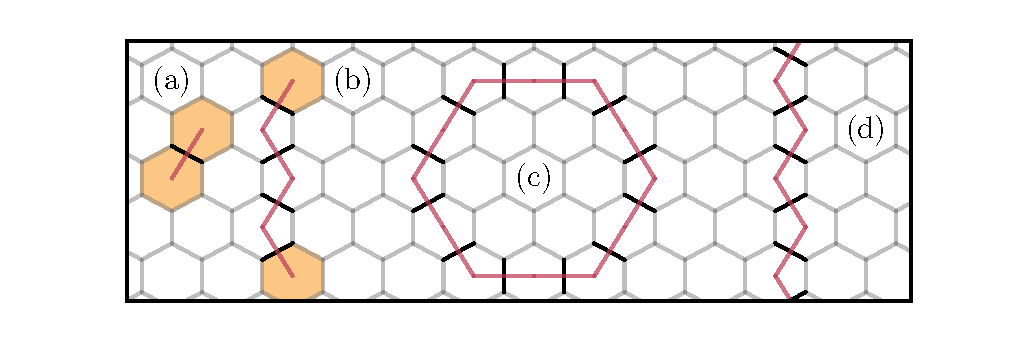
\includegraphics[width=1\textwidth,height=\textheight]{figure_code/amk_chapter/intro/types_of_dual_loops_animated/types_of_dual_loops_animated.pdf}
\caption{\textbf{Dual Loops and Vortex Pairs} The different kinds of strings and loops that we can make by flipping bond variables or transporting vortices around. (a) Flipping a single bond makes a pair of vortices on either side. (b) Flipping a string of bonds separates the vortex pair spatially. The flipped bonds form a path (in red) on the dual lattice. (c) If we create a vortex-vortex pair, transport one of them around a loop and then annihilate them, we can change the bond sector without changing the vortex sector. This is a manifestation of the gauge symmetry of the bond sector. (d) If we transport a vortex around the major or minor axes of the torus, we create a non-contractable loop of bonds \(\hat{\mathcal{T}}_{x/y}\). Unlike all the other dual loops, These operators cannot be constructed from the contractable loops created by \(D_j\). operators and they flip the value of the topological fluxes. \href{http://thomashodson.com/assets/thesis/figure_code/amk_chapter/intro/types_of_dual_loops_animated/types_of_dual_loops_animated.gif}{ Animated version online.}}\label{fig:types_of_dual_loops_animated}
}
\end{figure}

See \cref{fig:types_of_dual_loops_animated} for a diagram of the next three paragraphs.

We started from the ground state of the model and flipped the sign of a single bond (\cref{fig:types_of_dual_loops_animated} (a)). In doing so, we will flip the sign of the two plaquettes adjacent to that bond. We will call these disturbed plaquettes \emph{vortices}. We will refer to a particular choice values for the plaquette operators as a \emph{vortex sector}.

If we chain multiple bond flips, we can create a pair of vortices at arbitrary locations (\cref{fig:types_of_dual_loops_animated} (b)). The chain of bonds that we must flip corresponds to a path on the dual of the lattice.

We can also create a pair of vortices, move one around a loop and finally annihilate it with its partner (\cref{fig:types_of_dual_loops_animated} (c)). This corresponds to a closed loop on the dual lattice. Applying such a bond flip leaves the vortex sector unchanged. We can also do the same thing but move the vortex around one the non-contractible loops of the lattice (\cref{fig:types_of_dual_loops_animated} (d)).

\hypertarget{dual-loops-and-gauge-symmetries}{%
\subsubsection{Dual Loops and gauge symmetries}\label{dual-loops-and-gauge-symmetries}}

\begin{figure}
\hypertarget{fig:gauge_symmetries}{%
\centering
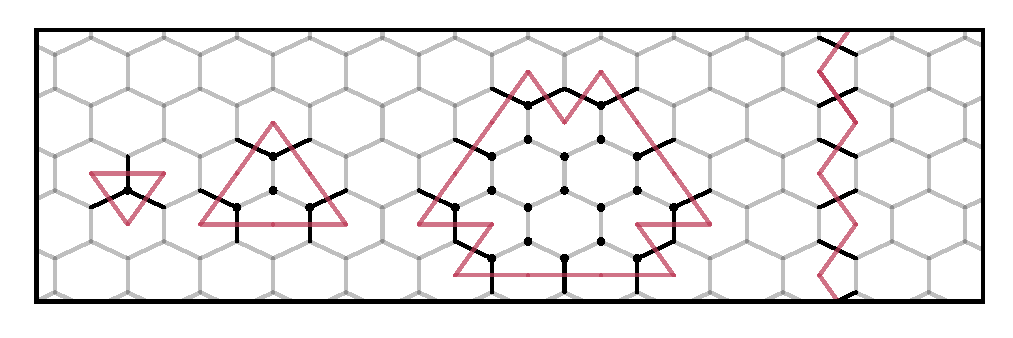
\includegraphics[width=1\textwidth,height=\textheight]{figure_code/amk_chapter/intro/gauge_symmetries/gauge_symmetries.pdf}
\caption{\textbf{Dual Loops and Gauge Symmetries} A honeycomb lattice with edges in light grey, along with its dual, the triangle lattice in light blue. The vertices of the dual lattice are the faces of the original lattice and, hence, are the locations of the vortices. (Left) The action of the gauge operator \(D_j\) at a vertex is to flip the value of the three \(u_{jk}\) variables (black lines) surrounding site \(j\). The corresponding edges of the dual lattice (red lines) form a closed triangle. (Middle) Composing multiple adjacent \(D_j\) operators produces a large closed dual loop or multiple disconnected dual loops. Dual loops are not directed like Wilson loops. (Right) A non-contractable loop which cannot be produced by composing \(D_j\) operators. All three operators can be thought of as the action of a vortex-vortex pair that is created, one of them is transported around the loop, and then the two annihilate again. Note that every plaquette has an even number of \(u_{ij}\)s flipped on its edge. Therefore, all retain the same value.}\label{fig:gauge_symmetries}
}
\end{figure}

See \cref{fig:gauge_symmetries} for a diagram of the next few paragraphs.

Notice that the \(D_j\) operators flip three bonds around a vertex. This is the smallest dual loop around which one can move a vortex pair and then annihilate it with itself.

Such operations compose, so we can build any larger loop (almost) by applying a series of \(D_j\) operations. The symmetrisation procedure \(\prod_i \left( \frac{1 + D_i}{2}\right)\) that maps from the bond sector to a physical state is really constructing a superposition over every such dual loops that leaves the vortex sector unchanged.

There is one kind of dual loop that we cannot build out of \(D_j\)s, the non-contractible loops.

\textbf{The plaquette operators and topological fluxes are the gauge invariant quantities which determine the physics of the model}

\hypertarget{composition-of-wilson-loops}{%
\subsubsection{Composition of Wilson loops}\label{composition-of-wilson-loops}}

\begin{figure}
\hypertarget{fig:plaquette_addition_by_hand}{%
\centering
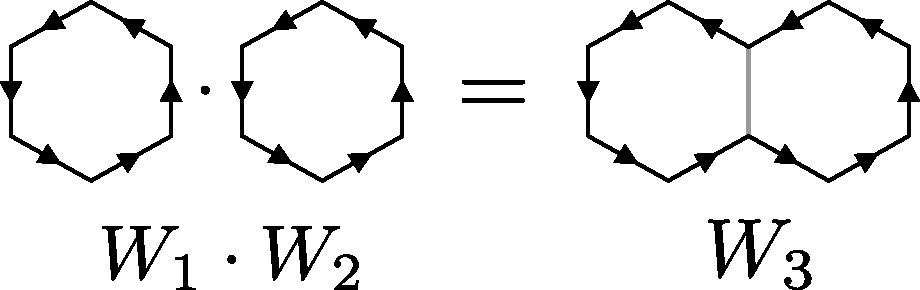
\includegraphics[width=0.57\textwidth,height=\textheight]{figure_code/amk_chapter/plaquette_addition/plaquette_addition_by_hand.pdf}
\caption{In the product of individual plaquette operators, shared bonds cancel out. The product is equal to the enclosing path.}\label{fig:plaquette_addition_by_hand}
}
\end{figure}

Second, one can now easily show that the loops and plaquettes satisfy nice composition rules, so long as we keep to loops that wind in a particular direction.

Consider the product of two non-overlapping loops \(W_a\) and \(W_b\) that share an edge \(u_{12}\). Since the two loops both wind clockwise and do not overlap, one will contain a term \(i u_{12}\) and the other \(i u_{21}\). Since the \(u_{ij}\) commute with one another, they square to \(1\) and \(u_{ij} = -u_{ji}\), we have \(i u_{12} i u_{21} = 1\). We can repeat this for any number of shared edges. Hence, we get a version of Stokes' theorem: the product of \(i u_{jk}\) around any closed loop \(\partial A\) is equal to the product of plaquette operators \(\Phi\) that span the area \(A\) enclosed by that loop: \[\prod_{u_{jk} \in \partial A} i \; u_{jk} = \prod_{\phi_i \in A} \phi_i\]

\begin{figure}
\hypertarget{fig:stokes_theorem}{%
\centering
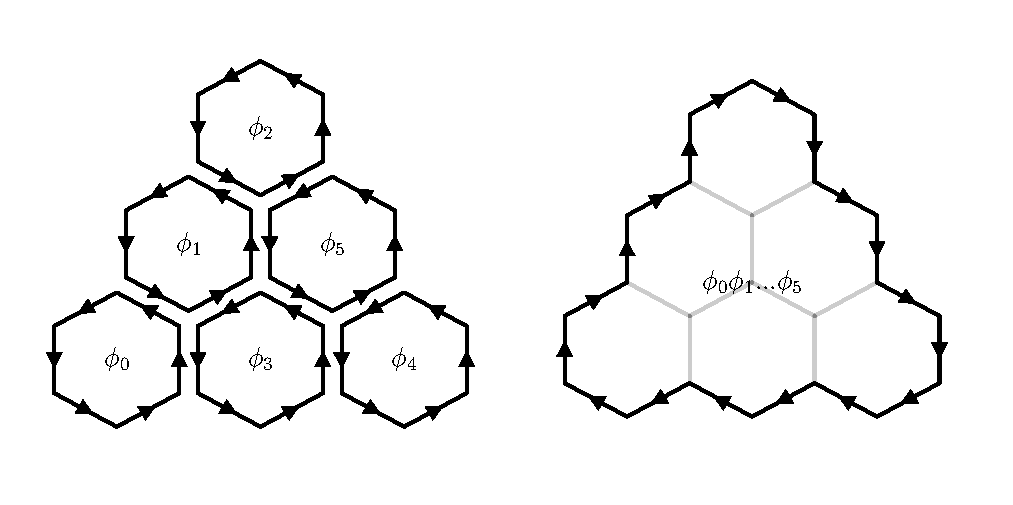
\includegraphics[width=0.71\textwidth,height=\textheight]{figure_code/amk_chapter/stokes_theorem/stokes_theorem.pdf}
\caption{The loop composition rule extends to arbitrary numbers of vortices which gives a discrete version of Stoke's theorem.}\label{fig:stokes_theorem}
}
\end{figure}

Takeaway: Wilson loops can always be decomposed into products of plaquettes operators unless they are non-contractable.

\hypertarget{gauge-degeneracy-and-the-euler-equation}{%
\subsubsection{Gauge Degeneracy and the Euler Equation}\label{gauge-degeneracy-and-the-euler-equation}}

\begin{figure}
\hypertarget{fig:state_decomposition_animated}{%
\centering
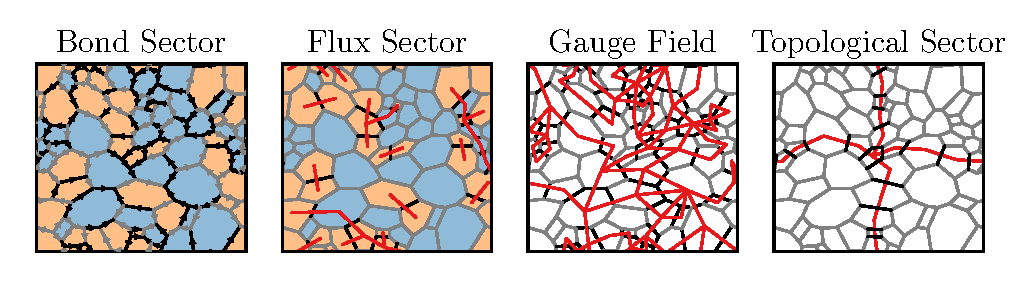
\includegraphics[width=1\textwidth,height=\textheight]{figure_code/amk_chapter/state_decomposition_animated/state_decomposition_animated.pdf}
\caption{(Bond Sector) A state in the bond sector is specified by assigning \(\pm 1\) to each edge of the lattice. However, this description has a substantial gauge degeneracy. We can simplify things by decomposing each state into the product of three kinds of objects: (Vortex Sector) Only a small number of bonds need to be flipped (compared to some arbitrary reference) to reconstruct the vortex sector. Here, the edges are chosen from a spanning tree of the dual lattice, so there are no loops. (Gauge Field) The `loopiness' of the bond sector can be factored out. This gives a network of loops that can always be written as a product of the gauge operators \(D_j\). (Topological Sector) Finally, there are two loops that have no effect on the vortex sector, nor can they be constructed from gauge symmetries. These can be thought of as two fluxes \(\Phi_{x/y}\) that thread through the major and minor axes of the torus. Measuring \(\Phi_{x/y}\) amounts to constructing Wilson loops around the axes of the torus. We can flip the value of \(\Phi_{x}\) by transporting a vortex pair around the torus in the \(y\) direction, as shown here. In each of the three figures on the right, black bonds correspond to those that must be flipped. Composing the three together gives back the original bond sector on the left. \href{http://thomashodson.com/assets/thesis/figure_code/amk_chapter/state_decomposition_animated/state_decomposition_animated.gif}{ Animated version online.}}\label{fig:state_decomposition_animated}
}
\end{figure}

We can check this analysis with a counting argument. For a lattice with \(B\) bonds, \(P\) plaquettes and \(V\) vertices, we can count the number of bond sectors, vortices sectors and gauge symmetries and check them against Euler's polyhedra equation.

Euler's equation states for a closed surface of genus \(g\), i.e that has \(g\) holes so \(0\) for the sphere, \(1\) for the torus and \(g\) for \(g\) tori stuck together \[B = P + V + 2 - 2g\]

\begin{figure}
\hypertarget{fig:torus}{%
\centering
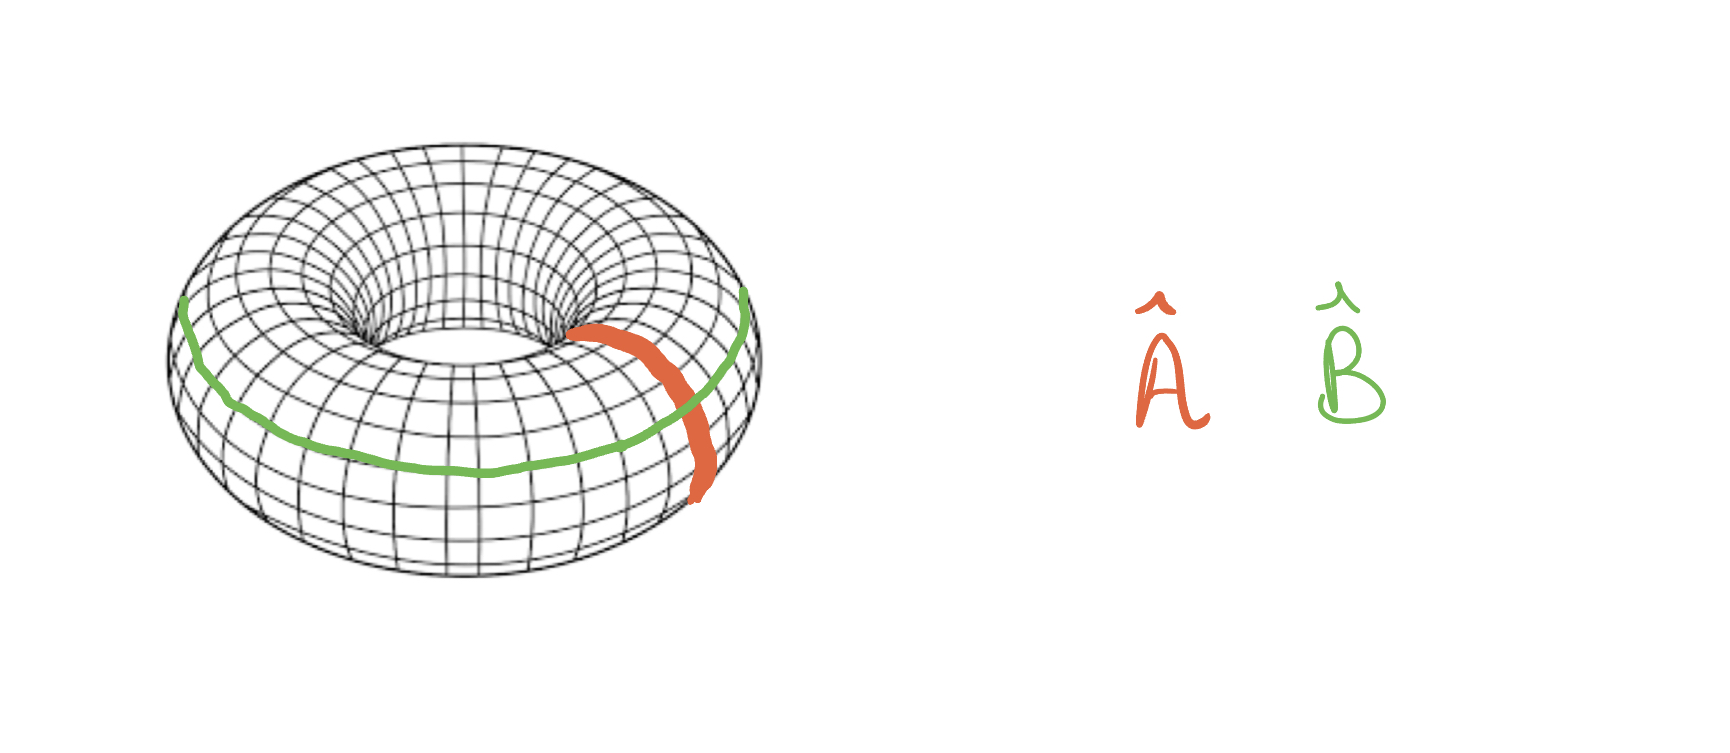
\includegraphics[width=0.86\textwidth,height=\textheight]{figure_code/amk_chapter/torus.jpeg}
\caption{In periodic boundary conditions the Kitaev model is defined on the surface of a torus. Topologically, the torus is distinct from the sphere in that it has a hole that cannot be smoothly deformed away. Associated with each such hole are two non-contractible loops on the surface, here labelled \(x\) and \(y\), which cannot be smoothly deformed to a point. These two non-contractible loops can be used to construct two special pairs of operators: The two topological fluxes \(\Phi_x\) and \(\Phi_y\) that are the expectation values of \(u_{jk}\) loops around each path. There are also two operators \(\hat{\mathcal{T}}_x\) and \(\hat{\mathcal{T}}_y\) that transform one half of a vortex pair around the loop before annihilating them together again, see later.}\label{fig:torus}
}
\end{figure}

For the case of the torus where \(g = 1\), we can rearrange this to read: \[B = (P-1) + (V-1) + 2\]

\textbf{Bond Sectrors}: Each \(u_{ij}\) takes two values and there is one associated with each bond so there are exactly \(2^B\) distinct configurations of the bond sector. Let us see if we can factor those configurations out into the Cartesian product of vortex sectors, gauge symmetries and non-contractible loop operators.

\textbf{Vortex sectors}: Each plaquette operator \(\phi_i\) takes two values (\(\pm 1\) or \(\pm i\)) and there are \(P\) of them. Vortices can only be created in pairs so there are \(\tfrac{2^P}{2} = 2^{P-1}\) vortex sectors in total. Denoting the number of pairs of vortices as \(N_v\), the vortex parity \(1 - 2*(N_v \mod 2)\) will be relevant in the projector later.

\textbf{Gauge symmetries}: As discussed earlier, these correspond to all possible compositions of the \(D_j\) operators. Again, there are only \(2^{V-1}\) of these because, as we will see in the next section, \(\prod_{j} D_j = \mathbb{1}\) in the physical space. We enforce this by choosing the correct product of single particle fermion states. One can get an intuitive picture for why \(\prod_{j} D_j = \mathbb{1}\) by imagining larger and larger patches of \(D_j\) operators on the torus. These patches correspond to transporting a vortex pair around the edge of the patch. At some point, the patch wraps around and starts to cover the entire torus. As this happens, the boundary of the patch disappears and, hence, it corresponds to the identity operation. See \cref{fig:flood_fill} and \cref{fig:flood_fill_amorphous}.

\textbf{Topological Sectors}: Finally, the torus has two non-contractible loop operators associated with its major and minor diameters. These give us two extra fluxes \(\Phi_x\) and \(\Phi_y\) each with two distinct values.

Putting this all together, we see that there are \textbf{\(2^B\) bond sectors} a space which can be decomposed into the Cartesian product of \textbf{\(2^{P-1}\) vortex sectors}, \textbf{\(2^{V-1}\) gauge symmetries} and \textbf{\(2^2 = 4\) topological sectors}.

The topological sector forms the basis of proposals to construct topologically protected qubits since the four sectors can only be mixed by a highly non-local perturbations \textcite{kitaevFaulttolerantQuantumComputation2003}.

Takeaway: The Extended Hilbert Space decomposes into a direct product of Flux Sectors, four Topological Sectors and a set of gauge symmetries.

\begin{figure}
\hypertarget{fig:flood_fill}{%
\centering
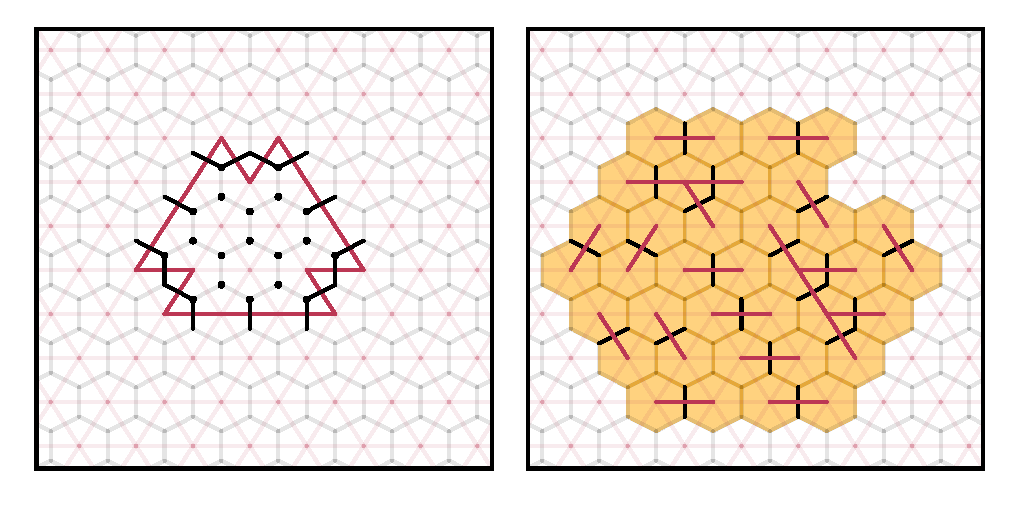
\includegraphics[width=1\textwidth,height=\textheight]{figure_code/amk_chapter/intro/flood_fill/flood_fill.pdf}
\caption{A honeycomb lattice (in black) along with its dual (in red). (Left) Taking a larger and larger set of \(D_j\) operators (Bold Vertices) leads to an outward expanding boundary dual loop. Eventually every lattice on the torus is included and the boundary contracts to a point and disappears. This is a visual proof that \(\prod_i D_i \propto \mathbb{1}\). We'll see later that it takes values \(\pm 1\) and is a key part of the projection to the physical subspace. (Right) In black and red the edges and dual edges that must be flipped to add vortices at the sites highlighted in orange. Flipping all the \emph{plaquettes} in the system is \textbf{not} equivalent to the identity. Not that the edges that must be flipped can always be chosen from a tree since loops can be removed by a gauge transformation. \href{http://thomashodson.com/assets/thesis/figure_code/amk_chapter/intro/flood_fill/flood_fill.gif}{ Animated version online.}}\label{fig:flood_fill}
}
\end{figure}

\hypertarget{counting-edges-plaquettes-and-vertices}{%
\subsubsection{Counting edges, plaquettes and vertices}\label{counting-edges-plaquettes-and-vertices}}

It is useful to know how the trivalent structure of the lattice constrains the number of bonds \(B\), plaquettes \(P\) and vertices \(V\) it has.

The lattice is built from vertices that each share three edges with their neighbours. This means that each vertex comes with \(\tfrac{3}{2}\) bonds i.e \(3V = 2B\). This is consistent with the fact that, in the Majorana representation on the torus, each vertex brings three \(b^\alpha\) operators which then pair along bonds to give \(3/2\) bonds per vertex.

If we define an integer \(N\) such that \(V = 2N\) and \(B = 3N\) and substitute this into the polyhedra equation for the torus, we see that \(P = N\). Therefore, if a trivalent lattice on the torus has \(N\) plaquettes, it has \(2N\) vertices and \(3N\) bonds.

We can also consider the sum of the number of bonds in each plaquette \(S_p\), since each bond is a member of exactly two plaquettes \[S_p = 2B = 6N\]

The mean size of a plaquette in a trivalent lattice on the torus is exactly six. As the sum is even, this also tells us that all odd plaquettes must come in pairs.

\begin{figure}
\hypertarget{fig:flood_fill_amorphous}{%
\centering
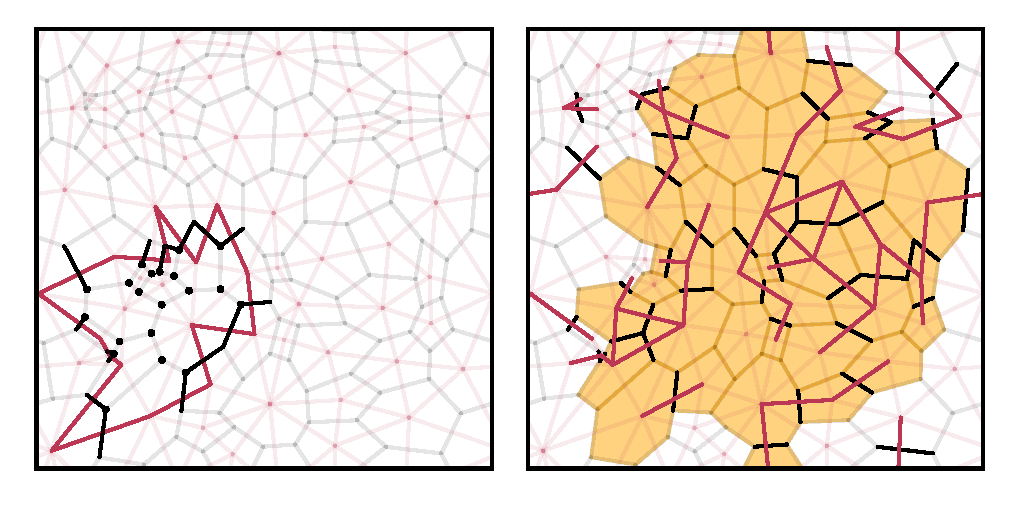
\includegraphics[width=1\textwidth,height=\textheight]{figure_code/amk_chapter/intro/flood_fill_amorphous/flood_fill_amorphous.pdf}
\caption{The same as \cref{fig:flood_fill} but for the amorphous lattice. \href{http://thomashodson.com/assets/thesis/figure_code/amk_chapter/intro/flood_fill_amorphous/flood_fill_amorphous.gif}{ Animated version online.}}\label{fig:flood_fill_amorphous}
}
\end{figure}

\hypertarget{the-projector}{%
\subsection{The Projector}\label{the-projector}}

The projection from the extended space to the physical space will not be particularly important for the results presented here. However, the theory remains useful to explain why this is.

\begin{figure}
\hypertarget{fig:hilbert_spaces}{%
\centering
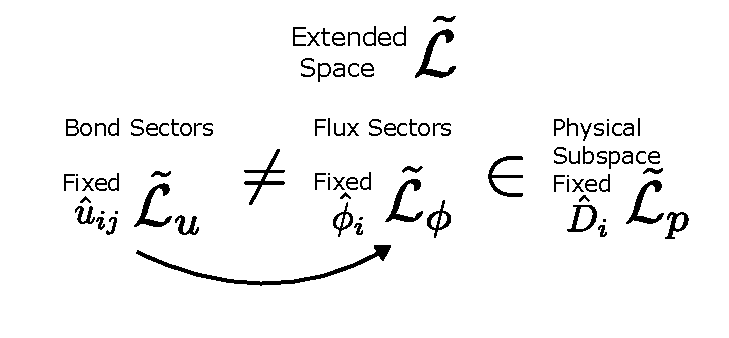
\includegraphics[width=1\textwidth,height=\textheight]{figure_code/amk_chapter/hilbert_spaces.pdf}
\caption{The relationship between the different Hilbert spaces used in the solution. \textbf{needs updating}}\label{fig:hilbert_spaces}
}
\end{figure}

The physical states are defined as those for which \(D_i |\phi\rangle = |\phi\rangle\) for all \(D_i\). Since \(D_i\) has eigenvalues \(\pm1\), the quantity \(\tfrac{(1+D_i)}{2}\) has eigenvalue \(1\) for physical states and \(0\) for extended states so is the local projector onto the physical subspace.

Therefore, the global projector is \[ \mathcal{P} = \prod_{i=1}^{2N} \left( \frac{1 + D_i}{2}\right)\]

for a toroidal trivalent lattice with \(N\) plaquettes \(2N\) vertices and \(3N\) edges. As discussed earlier, the product over \((1 + D_j)\) can also be thought of as the sum of all possible subsets \(\{i\}\) of the \(D_j\) operators, which is the set of all possible gauge symmetry operations.

\[ \mathcal{P} = \frac{1}{2^{2N}} \sum_{\{i\}} \prod_{i\in\{i\}} D_i\]

Since the gauge operators \(D_j\) commute and square to one, we can define the complement operator \(C = \prod_{i=1}^{2N} D_i\) and see that it takes each set of \(\prod_{i \in \{i\}} D_j\) operators and gives us the complement of that set. We will shortly see why \(C\) is the identity in the physical subspace, as noted earlier.

We use the complement operator to rewrite the projector as a sum over half the subsets of \(\{i\}\) - referred to as \(\Lambda\). The complement operator deals with the other half

\[ \mathcal{P} =  \left( \frac{1}{2^{2N-1}} \sum_{\Lambda} \prod_{i\in\{i\}} D_i\right) \left(\frac{1 + \prod_i^{2N} D_i}{2}\right) = \mathcal{S} \cdot \mathcal{P}_0\]

To compute \(\mathcal{P}_0\), the main quantity needed is the product of the local projectors \(D_i\) \[\prod_i^{2N} D_i = \prod_i^{2N} b^x_i b^y_i b^z_i c_i \] for a toroidal trivalent lattice with \(N\) plaquettes \(2N\) vertices and \(3N\) edges.

First, we reorder the operators by bond type. This does not require any information about the underlying lattice.

\[\prod_i^{2N} D_i = \prod_i^{2N} b^x_i \prod_i^{2N} b^y_i \prod_i^{2N} b^z_i \prod_i^{2N} c_i\]

The product over \(c_i\) operators reduces to a determinant of the Q matrix and the fermion parity, see \textcite{pedrocchiPhysicalSolutionsKitaev2011b}. The only difference from the honeycomb case is that we cannot explicitly compute the factors \(p_x,p_y,p_z = \pm\;1\) that arise from reordering the b operators such that pairs of vertices linked by the corresponding bonds are adjacent.

\[\prod_i^{2N} b^\alpha_i = p_\alpha \prod_{(i,j)}b^\alpha_i b^\alpha_j\]

However, they are simply the parity of the permutation from one ordering to the other and can be computed in linear time with a cycle decomposition \textcite{app:cycle_decomp}.

We find that \[\mathcal{P}_0 = 1 + p_x\;p_y\;p_z\; \hat{\pi} \; \mathrm{det}(Q^u) \; \prod_{\{i,j\}} -iu_{ij}\]

where \(p_x\;p_y\;p_z = \pm 1\) are lattice structure factors and \(\mathrm{det}(Q^u)\) is the determinant of the matrix mentioned earlier that maps \(c_i\) operators to normal mode operators \(b'_i, b''_i\). These depend only on the lattice structure.

\(\hat{\pi} = \prod{i}^{N} (1 - 2\hat{n}_i)\) is the parity of the particular many body state determined by fermionic occupation numbers \(n_i\). As discussed in +\textcite{pedrocchiPhysicalSolutionsKitaev2011b}, \(\hat{\pi}\) is gauge invariant in the sense that \([\hat{\pi}, D_i] = 0\).

This implies that \(det(Q^u) \prod -i u_{ij}\) is also a gauge invariant quantity. In translation invariant models this quantity which can be related to the parity of the number of vortex pairs in the system \textcite{yaoAlgebraicSpinLiquid2009}. I am unsure if this is true for the amorphous case.

All these factors take values \(\pm 1\) so \(\mathcal{P}_0\) is 0 or 1 for a particular state. Since \(\mathcal{S}\) corresponds to symmetrising over all the gauge configurations and cannot be 0, once we have determined the single particle eigenstates of a bond sector, the true many body ground state has the same energy as either the empty state with \(n_i = 0\) or a state with a single fermion in the lowest level.

\hypertarget{ground-state-degeneracy}{%
\subsubsection{Ground State Degeneracy}\label{ground-state-degeneracy}}

\begin{figure}
\hypertarget{fig:loops_and_dual_loops}{%
\centering
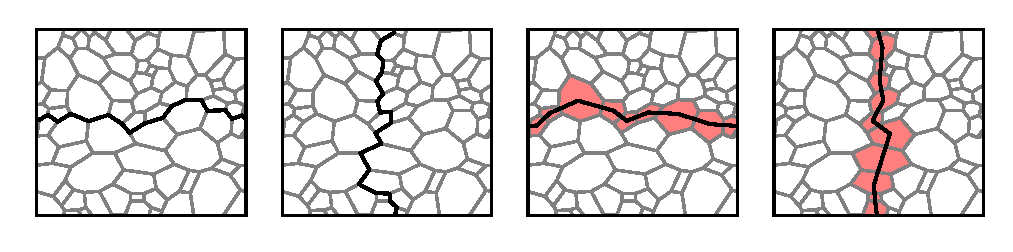
\includegraphics[width=1\textwidth,height=\textheight]{figure_code/amk_chapter/loops_and_dual_loops/loops_and_dual_loops.pdf}
\caption{(Left) The two topological flux operators of the toroidal lattice. These do not correspond to any face of the lattice, but rather measure flux that threads through the major and minor axes of the torus. This shows a particular choice. Yet, any loop that crosses the boundary is gauge equivalent to one of or the sum of these two loop. (Right) The two ways to transport vortices around the diameters. These amount to creating a vortex pair, transporting one of them around the major or minor diameters of the torus and, then, annihilating them again.}\label{fig:loops_and_dual_loops}
}
\end{figure}

More general arguments\autocite{chungExplicitMonodromyMoore2007,oshikawaTopologicalDegeneracyNonAbelian2007} imply that \(det(Q^u) \prod -i u_{ij}\) has an interesting relationship to the topological fluxes. In the non-Abelian phase, we expect that it will change sign in exactly one of the four topological sectors.

This means that the lowest state in three of the topological sectors contain no fermions, while in one of them there must be one fermion to preserve product of fermion vortex parity. So overall the non-Abelian model has a three-fold degenerate ground state rather than the fourfold of the Abelian case (and of my intuition!). In the Abelian phase, this does not happen and we get a fourfold degenerate ground state. Whether this analysis generalises to the amorphous case is unclear.

An alternative way to view this is to imagine we start in one state of the ground state manifold. We then attempt to construct other ground states by creating vortex pairs, transporting one vortex around one or both non-contractible loops and then annihilating them. This works for either of the two non-contractible loops but when we try to do it for \emph{both} something strange happens. When we transport a vortex around \textbf{both} the major and minor axes of the torus this changes its fusion channel. Normally two vortices fuse to the vacuum but after this operation they fuse into a fermion excitation. And hence our attempt to construct that last ground state doesn't yield a ground state at all, leaving us with just three.

\textbf{NOTE to self: This argument seems to involve adiabatic insertion of the fluxes \(\Phi_{x,y}\) as the operations that undo vortex transport around the lattice. I don't understand why that part is necessary}

\begin{figure}
\hypertarget{fig:threefold_degeneracy}{%
\centering
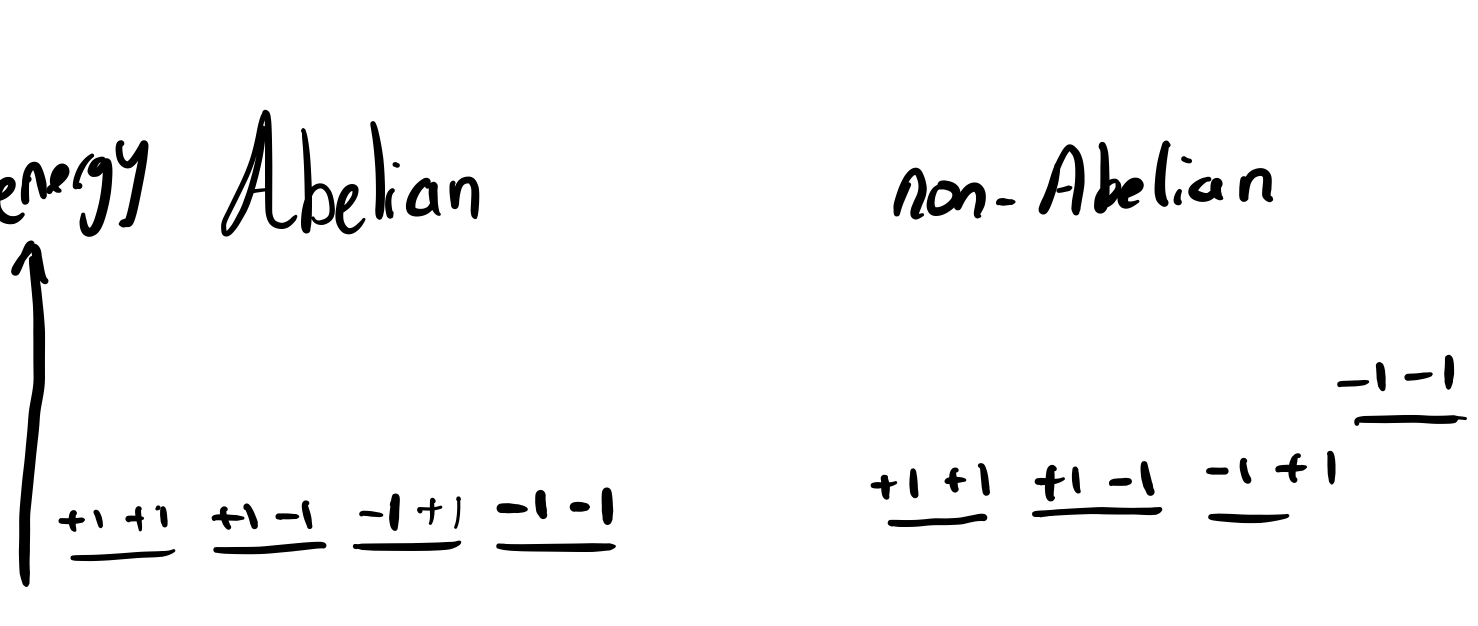
\includegraphics[width=0.86\textwidth,height=\textheight]{figure_code/amk_chapter/threefold_degeneracy.png}
\caption{In the non-Abelian phase one of the lowest energy state in one of the topological sectors contains a fermion and hence is slightly higher in energy than the other three. This manifests as a fourfold ground state degeneracy in the Abelian phase and a threefold degeneracy in the non-Abelian phase.}\label{fig:threefold_degeneracy}
}
\end{figure}

\hypertarget{quick-breather}{%
\subsubsection{Quick Breather}\label{quick-breather}}

Let's consider where are with the model now. We can map the spin Hamiltonian to a Majorana Hamiltonian in an extended Hilbert space. Along with that mapping comes a gauge field \(u_{jk}\) defining \textbf{bond sectors}. The gauge symmetries of \(u_{jk}\) are generated by the set of \(D_j\) operators. The gauge invariant, and, therefore, physically, relevant variables are the plaquette operators \(\phi_i\) which define as a \textbf{vortex sector}. To solve the Majorana Hamiltonian, we must remove hats from the gauge field by restricting ourselves to a particular bond sector. At this stage, the Majorana Hamiltonian becomes non-interacting and we can solve it like any quadratic theory. This lets us construct the single particle eigenstates from which we can also construct many body states. Yet, the many body states constructed in this way are not in the physical subspace!

For the many body states within a particular bond sector, \(\mathcal{P}_0 = 0,1\) tells us which of those overlap with the physical sector.

We see that finding a state that has overlap with a physical state only ever requires the addition or removal of one fermion. There are cases where this can make a difference, but for most observables, such as ground state energy, this correction scales away as the number of fermions in the system grows.

If we wanted to construct a full many body wavefunction in the spin basis, we would need to include the full symmetrisation over the gauge fields. However, this was not necessary for any of the results that will be presented here.

\hypertarget{the-ground-state}{%
\subsection{The Ground State}\label{the-ground-state}}

We have shown that the Hamiltonian is gauge invariant. As a result, only the flux sector and the two topological fluxes affect the spectrum of the Hamiltonian. Thus, we can label the many body ground state by a combination of fluxes and fermionic occupation numbers.

By studying the projector, we saw that the fermionic occupation numbers of the ground state will always be either \(n_m = 0\) or \(n_0 = 1, n_{m>1} = 0\) because the projector only enforces combined vortex and fermion parity.

I refer to the flux sector that contains the ground state as the ground state flux sector. Recall that the excitations of the fluxes away from the ground ground state configuration are called \textbf{vortices}, so that the ground state flux sector is, by definition, the vortex free sector.

On the Honeycomb, Lieb's theorem implies that the ground state corresponds to the state where all \(u_{jk} = 1\). This implies that the flux free sector is the ground state sector \textcite{lieb_flux_1994}.

Lieb's theorem does not generalise easily to the amorphous case. However, we can get some intuition by examining the problem that will lead to a guess for the ground state. We will then provide numerical evidence that this guess is in fact correct.

Consider the partition function of the Majorana hamiltonian: \[ \mathcal{Z} = \mathrm{Tr}\left( e^{-\beta H}\right) = \sum_i \exp{-\beta \epsilon_i}\] At low temperatures \(\mathcal{Z} \approx \beta \epsilon_0\) where \(\epsilon_0\) is the lowest energy fermionic state.

How does the \(\mathcal{Z}\) depend on the Majorana hamiltonian? Expanding the exponential out gives \[ \mathcal{Z} = \sum_n \frac{(-\beta)^n}{n!} \mathrm{Tr(H^k)} \]

This makes for an interesting observation. The Hamiltonian is essentially a scaled adjacency matrix. An adjacency matrix being a matrix \(g_{ij}\) such that \(g_{ij} = 1\) if vertices \(i\) and \(j\) and joined by an edge and 0 otherwise.

Powers of adjacency matrices have the property that the entry \((g^n)_{ij}\) corresponds to the number of paths of length \(n\) on the graph that begin at site \(i\) and end at site \(j\). These include somewhat degenerate paths that go back on themselves.

Therefore, the trace of an adjacency matrix \[\mathrm{Tr}(g^n) = \sum_i (g^n)_{ii}\] counts the number of loops of size \(n\) that can be drawn on the graph.

Applying the same treatment to our Majorana Hamiltonian, we can interpret \(u_ij\) to equal 0 if the two sites are not joined by a bond and we put ourselves in the isotropic phase where \(J^\alpha = 1\) \[ \tilde{H}_{ij} =  \tfrac{1}{2} i u_{ij}\]

We then see that the trace of the nth power of H is a sum over Wilson loops of size \(n\) with an additional factor of \(2^{-n}\). We showed earlier that the Wilson loop operators can always be written as products of the plaquette operators that they enclose.

Lumping all the prefactors together, we will get something schematically like: \[ \mathcal{Z} = c_A \hat{A} + c_B \hat{B} + \sum_i c_i \hat{\phi}_i + \sum_{ij} c_{ij}  \hat{\phi}_i \hat{\phi}_j + \sum_{ijk} c_{ijk}  \hat{\phi}_i \hat{\phi}_j \hat{\phi}_k + ...\]

Where the \(c\) factors would be something like \[c_{ijk...} = \sum_n \tfrac{(-\beta)^n}{n!} \tfrac{1}{2^n} K_{ijk...}\] This is a sum over all loop lengths \(n\) with, for each, a combinatorial factor \(K_{ijk...}\) that counts how many ways exist to draw a loop of length \(n\) that only encloses plaquettes \(ijk...\).

We also have the pesky topological fluxes \(Phi_x\) and \(\Phi_y\). Again, the prefactors for these are very complicated. However, we can intuitively see that for larger and larger loops lengths, there will be a combinatorial explosion of possible ways that they appear in these sums. We know that explosion will be suppressed exponentially for sufficiently large system sizes but for practical lattices they cause significant finite size effects.

We do not have much hope of actually evaluating this for an amorphous lattice. However, we can guess that the ground state vortex sector might be a simple function of the side length of each plaquette.

The ground state of the Amorphous Kitaev Model is found by setting the flux through each plaquette \(\phi\) to be equal to \(\phi^{\mathrm{g.s.}}(n_{\mathrm{sides}})\)

\[\begin{aligned}
    \phi^{\mathrm{g.s.}}(n_{\mathrm{sides}}) = -(\pm i)^{n_{\mathrm{sides}}},
\end{aligned}\] where \(n_{\mathrm{sides}}\) is the number of edges that form each plaquette and the choice of sign gives a twofold chiral ground state degeneracy.

This conjecture is consistent with Lieb's theorem on regular lattices \autocite{lieb_flux_1994} and is supported by numerical evidence. As noted before, any flux that differs from the ground state is an excitation which we call a vortex.

\hypertarget{finite-size-effects}{%
\subsubsection{Finite size effects}\label{finite-size-effects}}

This guess only works for larger lattices. To rigorously test it, we would want to directly enumerate the \(2^N\) vortex sectors for a smaller lattice and check that the lowest state found is the vortex sector predicted by our conjecture.

To do this we tile an amorphous lattice as the unit cell of a periodic \(N\times N\) system. Bonds that originally crossed the periodic boundaries now connect adjacent unit cells. Using Bloch's theorem, the problem essentially reduces back to the single amorphous unit cell. However, now the edges that cross the periodic boundaries pick up a phase dependent on the crystal momentum \(\vec{q} = (q_x, q_y)\) and the lattice vector of the bond \(\vec{x} = (+1, 0, -1, +1, 0, -1)\). Assigning these lattice vectors to each bond is also a very convenient way to store and plot toroidal graphs.

This can then be solved using Bloch's theorem. For a given crystal momentum \(\textbf{q} \in [0,2\pi)^2\), we are left with a Bloch Hamiltonian, which is identical to the original Hamiltonian aside from an extra phase on edges that cross the periodic boundaries in the \(x\) and \(y\) directions, \[\begin{aligned}
    M_{jk}(\textbf{q}) =  \frac{i}{2} J^{\alpha} u_{jk} e^{i q_{jk}},\end{aligned}\] where \(q_{jk} = q_x\) for a bond that crosses the \(x\)-periodic boundary in the positive direction, with the analogous definition for \(y\)-crossing bonds. We also have \(q_{jk} = -q_{kj}\). Finally, \(q_{jk} = 0\) if the edge does not cross any boundaries at all. In essence, we are imposing twisted boundary conditions on our system. The total energy of the tiled system can be calculated by summing the energy of \(M( \textbf{q})\) for every value of \(\textbf{q}\).

With this technique, the finite size effects related to the non-contractible loop operators are removed with only a linear penalty in computation time compared to the exponential penalty paid by simply diagonalising larger lattices.

This technique verifies that \(\phi_0\) correctly predicts the ground state for hundreds of thousands of lattices with up to twenty plaquettes. For larger lattices, we verified that random perturbations around the predicted ground state never yield a lower energy state.

\hypertarget{chiral-symmetry}{%
\subsubsection{Chiral Symmetry}\label{chiral-symmetry}}

The discussion above shows that the ground state has a twofold \textbf{chiral} degeneracy which arises because the global sign of the odd plaquettes does not matter.

This happens because we have broken the time reversal symmetry of the original model by adding odd plaquettes \autocite{Chua2011,yaoExactChiralSpin2007,ChuaPRB2011,Fiete2012,Natori2016,Wu2009,Peri2020,WangHaoranPRB2021}.

Similarly to the behaviour of the original Kitaev model in response to a magnetic field, we get two degenerate ground states of different handedness. Practically speaking, one ground state is related to the other by inverting the imaginary \(\phi\) fluxes \autocite{yaoExactChiralSpin2007}.

\hypertarget{phases-of-the-kitaev-model}{%
\subsection{Phases of the Kitaev Model}\label{phases-of-the-kitaev-model}}

discuss the Abelian A phase / toric code phase / anisotropic phase

the isotropic gapless phase of the standard model

The isotropic gapped phase with the addition of a magnetic field

\hypertarget{what-is-so-great-about-two-dimensions}{%
\subsection{What is so great about two dimensions?}\label{what-is-so-great-about-two-dimensions}}

\hypertarget{topology-chirality-and-edge-modes}{%
\subsubsection{Topology, chirality and edge modes}\label{topology-chirality-and-edge-modes}}

Most thermodynamic and quantum phases studied can be characterised by a local order parameter. That is, a function or operator that only requires knowledge about some fixed sized patch of the system that does not scale with system size.

However, there are quantum phases that cannot be characterised by such a local order parameter. These phases are instead said to possess `topological order'.

One easily observable property of topological order is that the ground state degeneracy depends on the topology of the manifold that we put the system on to. This is referred to as topological degeneracy to distinguish it from standard symmetry breaking.

The Kitaev model is a good example. We have already looked at it defined on a graph that is embedded either into the plane or onto the torus. The extension to surfaces like the torus but with more than one handle is relatively easy.

\hypertarget{anyonic-statistics}{%
\subsubsection{Anyonic Statistics}\label{anyonic-statistics}}

\textbf{NB: I'm thinking about moving this section to the overall intro, but it's nice to be able to refer to specifics of the Kitaev model also so I'm not sure. It currently repeats a discussion of the ground state degeneracy from the projector section.}

In dimensions greater than two, the quantum state of a system must pick up a factor of \(-1\) or \(+1\) if two identical particles are swapped. We call these Fermions and Bosons.

This argument is predicated on the idea that performing two swaps is equivalent to doing nothing. Doing nothing should not change the quantum state at all. Therefore, doing one swap can at most multiply it by \(\pm 1\).

However, there are many hidden parts to this argument. First, this argument does not present the whole story. For instance, if you want to know why Fermions have half integer spin, you have to go to field theory.

Second, why does this argument only work in dimensions greater than two? When we say that two swaps do nothing, we in fact say that the world lines of two particles that have been swapped twice can be untangled without crossing. Why can't they cross? Because if they cross, the particles can interact and the quantum state could change in an arbitrary way. We are implicitly using the locality of physics to argue that, if the worldlines stay well separated, the overall quantum state cannot change.

In two dimensions, we cannot untangle the worldlines of two particles that have swapped places. They are braided together (see \cref{fig:braiding}).

\begin{figure}
\hypertarget{fig:braiding}{%
\centering
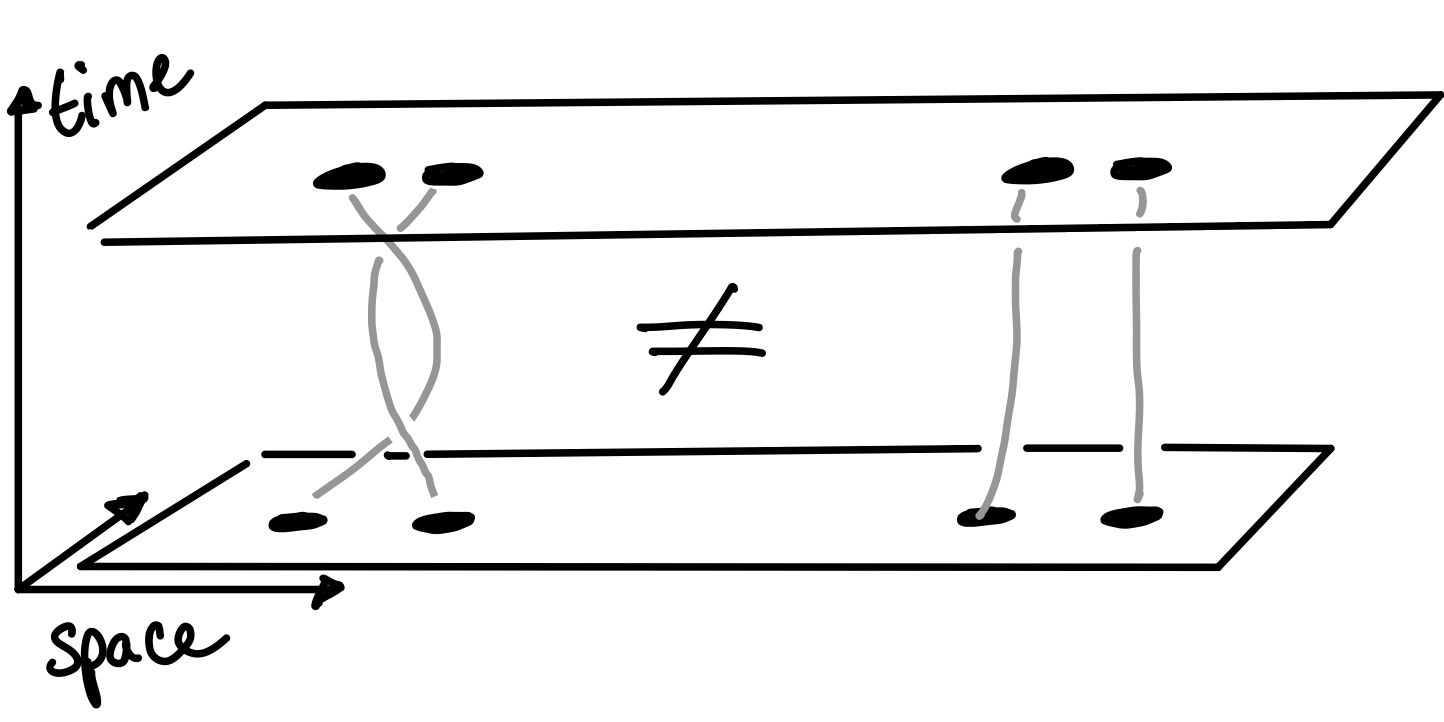
\includegraphics[width=0.71\textwidth,height=\textheight]{figure_code/amk_chapter/braiding.png}
\caption{Worldlines of particles in two dimensions can become tangled or \emph{braided} with one another.}\label{fig:braiding}
}
\end{figure}

From this fact flows a whole of behaviours. The quantum state can acquire a phase factor \(e^{i\phi}\) upon exchange of two identical particles, which we now call Anyons.

The Kitaev Model is a good demonstration of the connection between Anyons and topological degeneracy. In the Kitaev model, we can create a pair of vortices, move one around a non-contractable loop \(\mathcal{T}_{x/y}\) and then annihilate them together. Without topology, this should leave the quantum state unchanged. Instead, we move towards another ground state in a topologically degenerate ground state subspace. Practically speaking, it flips a dual line of bonds \(u_{jk}\) going around the loop which we cannot undo with any gauge transformation made from \(D_j\) operators.

If the ground state subspace is multidimensional, quasiparticle exchange can move us around in the space with an action corresponding to a matrix. In general, these matrices do not commute so these are known as non-Abelian anyons.

From here, the situation becomes even more complex. The Kitaev model has a non-Abelian phase when exposed to a magnetic field. The amorphous Kitaev Model has a non-Abelian phase because of its broken chiral symmetry.

By subdividing the Kitaev model into vortex sectors, we neatly separate between vortices and fermionic excitations. However, if we looked at the full many body picture, we would see that a vortex carries with it a cloud of bound Majorana states.

\begin{figure}
\hypertarget{fig:majorana_bound_states}{%
\centering
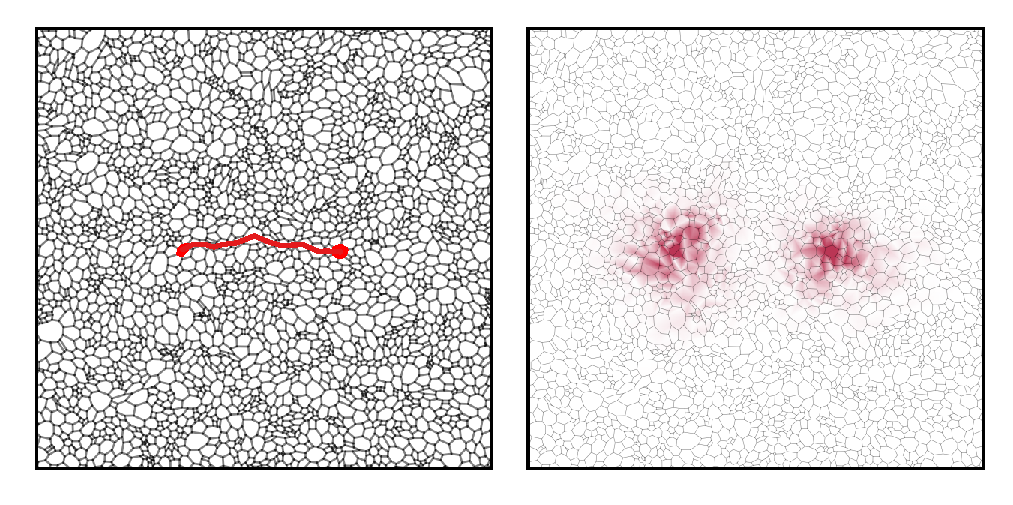
\includegraphics[width=1\textwidth,height=\textheight]{figure_code/amk_chapter/majorana_bound_states/majorana_bound_states.pdf}
\caption{(Left) A large amorphous lattice in the ground state save for a single pair of vortices shown in red, separated by the string of bonds that we flipped to create them. (Right) The density of the lowest energy Majorana state in this vortex sector. These Majorana states are bound to the vortices. They `dress' the vortices to create a composite object.}\label{fig:majorana_bound_states}
}
\end{figure}

Consider two processes

\begin{enumerate}
\def\labelenumi{\arabic{enumi})}
\item
  We transport one half of a vortex pair around either the x or y loops of the torus before annihilating back to the ground state vortex sector \(\mathcal{T}_{x,y}\).
\item
  We flip a line of bond operators corresponding to measuring the flux through either the major or minor axes of the torus \(\mathcal{\Phi}_{x,y}\)
\end{enumerate}

The plaquette operators \(\phi_i\) are associated with fluxes. Wilson loops that wind the torus are associated with the fluxes through its two diameters \(\mathcal{\Phi}_{x,y}\).

In the Abelian phase, we can move a vortex along any path at will before bringing them back together. They will annihilate back to the vacuum, where we understand `the vacuum' to refer to one of the ground states. However, this will not necessarily be the same ground state we started in. We can use this to get from the \((\Phi_x, \Phi_y) = (+1, +1)\) ground state and construct the set \((+1, +1), (+1, -1), (-1, +1), (-1, -1)\).

\begin{figure}
\hypertarget{fig:topological_fluxes}{%
\centering
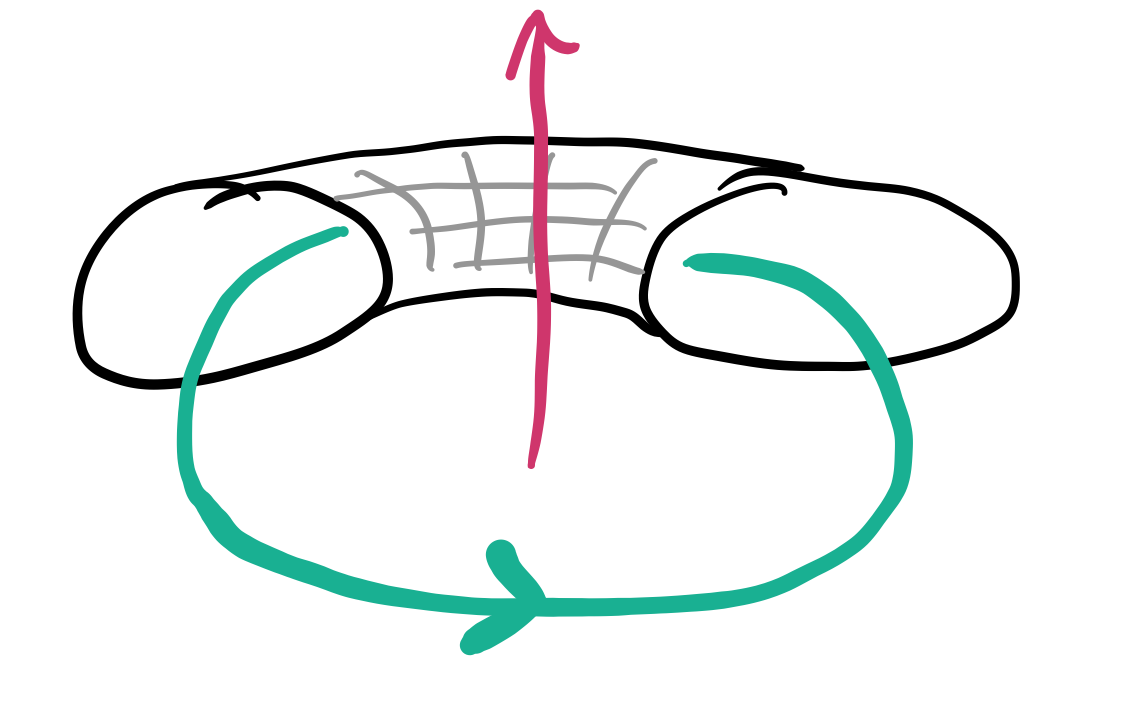
\includegraphics[width=0.57\textwidth,height=\textheight]{figure_code/amk_chapter/topological_fluxes.png}
\caption{Wilson loops that wind the major or minor diameters of the torus measure flux winding through the hole of the doughnut/torus or through the filling. If they made doughnuts that both had a jam filling and a hole, this analogy would be a lot easier to make \textcite{parkerWhyDoesThis}.}\label{fig:topological_fluxes}
}
\end{figure}

However, in the non-Abelian phase we have to wrangle with monodromy \autocite{chungExplicitMonodromyMoore2007,oshikawaTopologicalDegeneracyNonAbelian2007}. Monodromy is the behaviour of objects as they move around a singularity. This manifests here in that the identity of a vortex and cloud of Majoranas can change as we wind them around the torus in such a way that, rather than annihilating to the vacuum, we annihilate them to create an excited state instead of a ground state. This means that we end up with only three degenerate ground states in the non-Abelian phase \((+1, +1), (+1, -1), (-1, +1)\) \autocite[yaoAlgebraicSpinLiquid2009a]{chungTopologicalQuantumPhase2010}. Concretely, this is because the projector enforces both flux and fermion parity. When we wind a vortex around both non-contractible loops of the torus, it flips the flux parity. Therefore, we have to introduce a fermionic excitation to make the state physical. Hence, the process does not give a fourth ground state.

Recently, the topology has notably gained interest because of proposals to use this ground state degeneracy to implement both passively fault tolerant and actively stabilised quantum computations {[}\textcite{kitaevFaulttolerantQuantumComputation2003}; \textcite{poulinStabilizerFormalismOperator2005}; hastingsDynamicallyGeneratedLogical2021{]}.
